\section{Introduction}
\subsection{Background and Motivation}
Problem definition

=========================GWEN=========================
\begin{itemize}
    \item definition of NFC
    \item Quickness vs accuracy
    \item Depletion calculations for LWRs
    \item current practice for depletion calculations [citations]
    \item pros and cons of those practices [citations]
    \item Does it even matter? Fuel cycle simulation is a system-level analysis. How much does it matter? [citations]
\end{itemize}


\gls{NFC} simulations are system-level analyses that track
material flow in a \gls{NFC}. 

Since \gls{NFC} simulations
involve many facilities, the fidelity and detail of modeling each
facility are sacrificed for quickness. 

One of the most crucial functionalities in a \gls{NFC}
simulation is the transmutation of nuclear fuel in a reactor,
which is directly related to the \gls{UNF} composition
and waste / material profile.

Depletion calculations for fuel cycle simulations in current
\gls{NFC} simulators are either
recipe based (no calculation performed), 
library based, [so on and so forth, with citation].



1.The model approach predicts \gls{UNF} inventory far better than
the recipe approach, and takes into account the varying burnup and
enrichment.
2. The model approach can predict the composition of future
\gls{UNF} with higher burnup and enrichment [andrei]

=========================GWENEND=========================

\subsection{\Cyclus}

\Cyclus is an agent-based nuclear fuel cycle simulation framework 
\cite{huff_fundamental_2016}, meaning
that each reactor and fuel cycle facility is modeled as a discrete and independent
player in the simulation.
A \Cyclus agent archetype defines the logic that governs the behavior
of an agent. 
\Cyclus archetypes can be coded either with c++ or python.
In this simulation, the user defines the archetype's
parameters. The archetypes with user-defined parameters are then deployed
as agent prototypes.  Encapsulating the \texttt{Facility} agents are the \texttt{Institution} and \texttt{Region}.
A \texttt{Region} agent holds a set of \texttt{Institution}s. 
An \texttt{Institution} agent can deploy or decommission \texttt{Facility} agents.

At each timestep,
agents make requests for materials or bid to supply them and exchange
with one another. A market-like mechanism called the dynamic resource exchange
\cite{gidden_methodology_2016} governs the exchanges.
For output analysis, each material resource has a quantity, composition, name, and a unique identifier.

Cyclus has multiple advantages over other available
\gls{NFC} simulation codes including open-source distribution, modularity,
and extensibility. Its agent-based modeling approach
is ideal for modeling coupled, physics-dependent
supply chain problems common in \glspl{NFC}.
The framework allows for dynamic loading of 
external libraries, which allows the users to plug-and-play
different types of physics models for \gls{NFC}
simulation.


\subsubsection{Modularity and Extensibility}

In most modern \glspl{NFC} simulators, the facilities and their
behaviors (and their fidelities) are confined in the software.
Also, most modern \gls{NFC} simulators model
fuel cycles (once-through, continuous reprocessing)
with immutable connections between facilities. On the
other hand, \Cyclus allows users to plug-and-play various agent models
within the \Cyclus framework (shown in figure \ref{fig:core}).
Also, \Cyclus relies on a market-based model
for material trades between facilities, so the user can design
any novel fuel cycle. This enables \Cyclus to simulate any system analysis
involving multiple connected facilities with physics-based
calculations.


\begin{figure}[htbp!]
    \begin{center}
        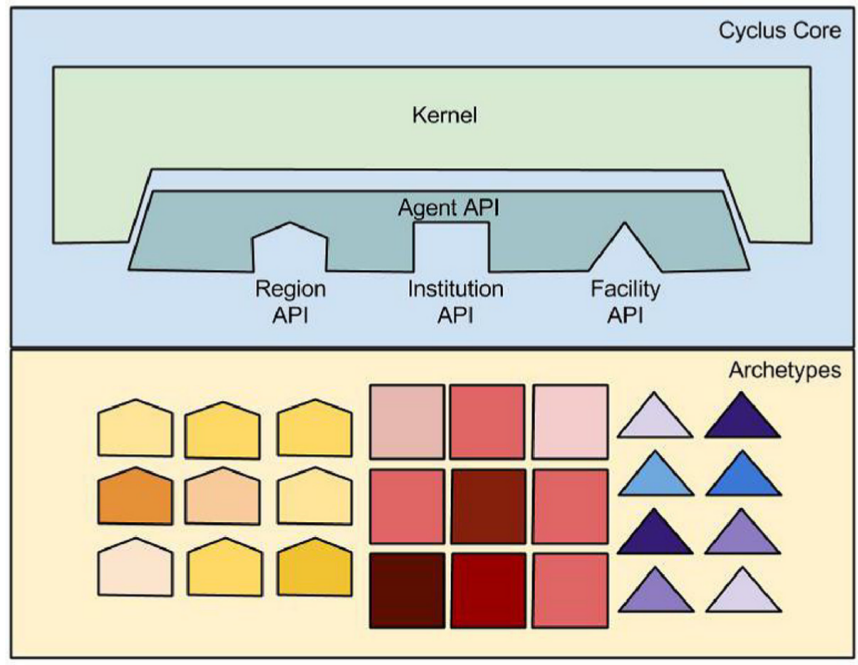
\includegraphics[width=\textwidth]{cyclus_core.png}
    \end{center}
    \caption{The \Cyclus core provides APIs that the archetypes
            can be loaded into the simulation modularly
            \cite{huff_fundamental_2016}.}
    \label{fig:core}
\end{figure}

Due to this modularity in the \Cyclus framework, the developed
model in this work can be implemented independently without
having to modify the \Cyclus source code. The new facility archetype
is simply written with the \Cyclus API, and imported in a
\Cyclus simulation.

\subsubsection{\Cycamore Recipe Reactor}
\Cycamore is a library that consists of useful
fuel cycle facility archetypes for \Cyclus. The
recipe reactor in \Cycamore is a batch-wise reactor.
A reactor core is consisted of multiple batches,
and a batch is consisted of multiple assemblies.
At startup, the reactor requests the entire core,
which is consisted of user-defined number of assemblies.
At every cycle, the reactor discharges and
requests batches of fuel. Upon decommissioning,
the reactor discharges all its fuel. The discharged
fuel is transmutated to the user-defined recipe.
No depletion calculation is performed. However,
the user can define multiple recipes, and can define
times to change the recipe from one to another.
